

\section{Funktion eines HF-Verstärkers}
Ein Verstärker ist ein elektronisches Gerät, mit mindestens einem 
aktiven Bauelement wie zum Beispiel einem Transistor.
Das Ziel eines Verstärkers ist dass,das Ausgangssignal 
größer als das Eingangssignal ist. Da hierbei dem Signal leistung hinzugefügt
wird muss ein Verstärker eine eigene Energie Quelle haben.
\\
Besonders in der Hochfrequenztechnik (HF) spielt der Verstärker eine wichtige
Rolle. Soll zum Beispiel mithilfe einer Antenna noch in weiter entfernung ein Signal
gemessen werden muss dies zuerst verstärkt werden.
\\
Normalerweise werdem im Hochfrequenzbereich Frequenzen von 10 kHZ bis 100.000ß MHz
verstärkt.
\clearpage
\section{Arbeitspunkeinstellung}
Der Arbeitspunkt einer elektronischen Schaltung beschreibt den 
Ruhezustand wenn kein Signal angelegt ist.
Er liegt auf einem bestimmten Punkt der Kennlinie.
Je nach einstellung kann die Schaltung anders auf das Eingangssignal
reagieren.
\\
\\
Einfache EmitterSchaltung:
\begin{figure}[h]
    \centering
    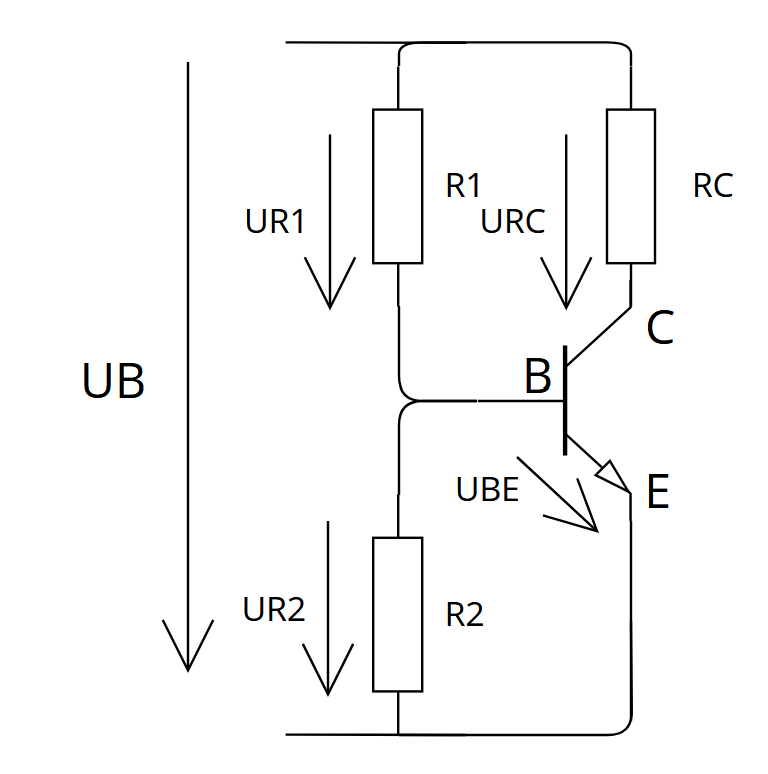
\includegraphics[width=0.6\textwidth]{Pictures/EmitterSchaltung.png}
    \caption{Emitterschaltung}
\end{figure}
\\
Gegebene Größen:
\begin{align}
    P_{saflj} : textsc
\end{align}
\section{Bedeutung der S-Parameter}
S-Parameter bzw. Streuparameter werden genutzt um die HF-Eigenschaften eines
Netzwerks darzustellen. Sie werden benötigt um zu verstehen welche Anteile eines Signals
reflektiert, durchgelassen oder zwischen den Toren eines Netzwerks übertragen werden.
Sie werden komplex dargestellt, also mit Betrags- und Phasenkomponente.
\\
Die Index numerierung folgt dem Energiefluss
\clearpage

\begin{itemize}
    \item verläuft die Energie von Tor 1 in Tor 1 heißt der S-Parameter S11
    \item verläuft die Energie von Tor 2 in Tor 1 heißt der S-Parameter S21
\end{itemize}
Somit können an einem Zweitor Folgende S-Parameter auftreten:
\begin{itemize}
    \item S11 ist der Eingangsreflexionsfaktor, Dieser Parameter gibt an wie viel des Eingangssignal zurückreflektiert wird.
    \item S21 ist der Vorwärtstransmissionsfaktor, Dieser Parameter gibt also die Effizienz der Signalübertragung vom Eingang zum Ausgang an.
    \item S12 ist der Rückwärtstransmissionsfaktor, Dieser Parameter gibt an wie gut Tor 1 von Signalen von Tor 2 isoliert ist.
    \item S22 ist der Ausgangsreflexionsfaktor, Dieser Parameter gibt an wie viel des Ausgangssignal zurückreflektiert wird.
\end{itemize}
\subsection{Smith-Diagramm}
Das Smith-Diagramm ermöglich die grafische Darstellung der S-Parameter.
Dafür wird der Real- und Imaginärteil des Reflexionsfaktor in abhängigkeit von der Frequenzen
aufgetragen und ermöglicht dadurch eine einfachere Impedanzanpassung.
\section{(rolle kopplungskodensator)}
blabla 
\clearpage